\documentclass[conference]{IEEEtran}
\IEEEoverridecommandlockouts
\usepackage{cite}
\usepackage{float}
\usepackage{amsmath,amssymb,amsfonts}
\usepackage{graphicx}
\usepackage{textcomp}
\usepackage[table]{xcolor}
\usepackage{booktabs}
\usepackage{array}
\usepackage{pifont}
\usepackage{tikz}
\usepackage[colorlinks=true,citecolor=blue,linkcolor=black,urlcolor=blue]{hyperref}
\usetikzlibrary{arrows.meta,fit,backgrounds}
\setlength{\textfloatsep}{7pt plus 2pt minus 2pt}
\setlength{\floatsep}{6pt plus 2pt minus 2pt}
\setlength{\intextsep}{6pt plus 2pt minus 2pt}
\newcommand{\yes}{\ding{51}}
\newcommand{\partl}{(\ding{51})}
\newcommand{\no}{--}
\newcommand{\so}{\texttt{success\_only}}
\newcommand{\ao}{\texttt{any\_outcome}}

\begin{document}

\title{Layer by Layer: An Empirical Ablation of\\Replay Defenses in a Signed Banking API}

% NOTE: if ECCE uses blind review, replace all author information with "Anonymous".

\author{
\IEEEauthorblockN{MD. Shahriar Islam}
\IEEEauthorblockA{
\textit{Department of CSE} \\
\textit{United International University} \\
Dhaka, Bangladesh \\
adsh257@gmail.com
}
\and
\IEEEauthorblockN{Md. Mine Uddin}
\IEEEauthorblockA{
\textit{Department of CSE} \\
\textit{United International University} \\
Dhaka, Bangladesh \\
md.mineuddin1212@gmail.com
}
\and
\IEEEauthorblockN{Maknun Ahmed Sifat}
\IEEEauthorblockA{
\textit{Department of CSE} \\
\textit{United International University} \\
Dhaka, Bangladesh \\
maknunsifat2002@gmail.com
}
}

\IEEEaftertitletext{%
\begin{center}
\footnotesize
\textit{MD. Shahriar Islam, Md. Mine Uddin, and Maknun Ahmed Sifat contributed equally to this work.}
\end{center}
}

\maketitle



\maketitle

\begin{abstract}
Replay attacks on signed transaction APIs are generally addressed using request signatures, timestamp windows, single-use nonces, and idempotency keys, but specifications do not mandate window sizes, nonce expiration times, and failure handling for requests. We analyze how these four layers combine on a repeatable banking API testbed with a ledger-based oracle for money movement. A 16-fold factorial ablation study of attack scenarios and layer configurations identifies which layer defends against which attack. The two most important findings are as follows. First, a layer of idempotency that remembers only successful requests does not protect from replaying previously failed requests because of the lack of funds; after transferring the money to the account, all 30 of such requests succeeded. Whereas the nonce check prevented fast replays and timestamp checks slow replays, the logging of every result prevents them both, albeit by disallowing retrying within the same ID. Also, nonce storage has to account for both past and future tolerance windows since the combination of default parameters (300 s nonce storage, 300 s past window, and 5 s future) allows for successful replay by the client clocked ahead of its time by 4 s within 301 s and 303 s. There is a total of about 0.5 ms per call on average for the four layers combined. All the results have been attained via single-machine simulations.
\end{abstract}

\begin{IEEEkeywords}
replay attack, HMAC, nonce, idempotency, defense in depth, transaction API
\end{IEEEkeywords}




\section{Introduction}\label{sec:intro}

Bank APIs offer the facility of transferring funds via HTTP requests. An attacker can intercept the request from a log, proxy, or TLS-termination gateway and replay the request so that the same transaction gets executed again. For example, a request for withdrawal of 1,000 BDT can be repeated. Although TLS protects information sent over the network, it does not eliminate the possibility of reusing an intercepted request. Replay attack is detrimental to the authentication and open banking protocols~\cite{gong92,rfc4120,almehrej,hosseyni24}.

One of the most widely used countermeasures involves four layers. The first layer involves the use of HMAC-SHA256 signatures to help identify the changes made to the signed fields of the request. The second layer is timestamps that limit the age of the request. The third layer in this countermeasure is single-use nonce which is used to determine whether a request has been repeated or not while keeping them in record. The fourth layer is the request ID (idempotency key) layer recorded in the ledger so that a repeated id is blocked or rejected.

The RFC document indicates the key specification related to nonce, signature age, and time window used in the application ~\cite{rfc9421}. The RFC 9449 is aimed at limiting the proof acceptance period and provides the replay-protection capabilities of different systems ~\cite{rfc9449}. The findings obtained after the analysis of financial-grade APIs demonstrate that no information about various timing and configuration issues discussed in the current research is available ~\cite{fett19,hosseyni24}. The researches concerned with idempotency focus on the issue of spontaneous duplicates ~\cite{lee15,whitaker25}.

The question concerning interaction of levels in different surroundings is not considered. The errors that happen while the levels are being skipped or when the states are being retained also help solving the problem related to replaying. The way the failed requests are treated also matters: v1 API returns the state while in v2 API the state gets retried~\cite{stripe}.

The case of S10 is an example of a replayed transaction. The same transaction is refused with respect to a certain account if it has insufficient funds in the account. In this case, the lesson is that if the state of the account is changed, then the same transaction can be executed now due to the fact that API accepts the same transaction request to be executed again, which was previously rejected. So, We address the following four research questions:

\begin{enumerate}
\item \textbf{RQ1 (Coverage):} What attacks can be deterred by each security layer on their own and in combination with other layers?

\item \textbf{RQ2 (Failed requests):} Is the policy for recording failed requests instrumental in determining whether the replay will succeed in case of change in the account state? Which security layers are needed to prevent the above-mentioned replays? 

\item \textbf{RQ3 (Nonce retention):} What is the relationship between nonce retention and asymmetric timestamp tolerance that allows different acceptance periods of time? 

\item \textbf{RQ4 (Operational effects):} What is the impact of nonce-store failure and clock skew on security and availability, and what is the cost of processing in the four security layers?

\end{enumerate}

In the experiment, Anis is the honest client performing normal withdrawals, while Eve is the attacker who captures and replays the client’s transaction requests. The contributions of this study are:

\begin{enumerate}
\item \textbf{Coverage of security layers (RQ1):} We examine the 16 possible combinations of the four security layers with respect to 11 attacks (13 variations). The coverage matrix derived indicates the level of each layer protection from the attacks, both on its own and together with others.

\item \textbf{Replay of failed requests (RQ2):} We determine the influence of a replay of failed requests in terms of idempotency policy alternatives.

\item \textbf{Nonce retention gap (RQ3):} We determine the nonce retention gap for default settings and a significant number of combinations. While the basic idea underlies RFC 9449, our effort is in measuring the exposure in the tested system.

\item \textbf{Operational behavior and costs (RQ4):} We quantify the impact of the nonce storage failures, missing responses, and clock drifts as well as false refusals and costs of processing.

\end{enumerate}



\section{Related Work}\label{sec:related}

\textbf{Standards and Formulations of Analysis.}
RFC 9449 has set a limit for the time of using DPoP proofs by servers, but it allows some future timestamps to take into account clock drift, and it promotes the use of new proofs at every attempt ~\cite{rfc9449}; RFC 9421 defines the parameters of \emph{created}, \emph{expires} and \emph{nonce}, while maximum age, nonce unique, and time windows parameters are determined by applications ~\cite{rfc9421}. Fett et al. conducted the four types of attacks against OpenID financial grade API and verified the fixed properties of the protocol ~\cite{fett19}. Hosseyni et al. modified this work on FAPI 2.0 using DPoP and signed messages, and finding even more attacks including the DPoP proofs replay attack~\cite{hosseyni24}. Both techniques leave timing parameters such as window sizes out of their models. Almehrej et al. have shown that it is possible to replay the previous replies in the Open Banking account protocol together with the usage of nonce to prevent this problem~\cite{almehrej}. Their research is about the logic of protocols only, without reference to the variables of windows of time or length of the failures.

\textbf{Replay defenses in the banking sector and their uses.}
The term “replay” is used by Jing et al. for the multiple instances of generating fraudulent transactions while processing 18 million bank transactions, as against the use of request replay~\cite{jing}. Arta mentions the usage of HMAC-SHA256, timestamps and Redis based nonces for the REST APIs causing an increase in latency of 0.453 ms on the same host ~\cite{arta}. Ibrahim and Alrajh claim the capability of detecting 10,000 replayed tokens in a multi-layer architecture and with constant token validity of 120 s ~\cite{ibrahim}. 

\textbf{Freshness, clocks and idempotency.}
The freshness of timestamps is dependent on synchronized clocks~\cite{gong92}. Kerberos uses timestamps in authenticators ~\cite{rfc4120}. Li et al. analyse timed protocols with parameters and identify a timing flaw in the specification of Kerberos V~\cite{li18}. Krentz and Voigt analyse differing types of freshness, sequential and strong freshness in context of limited resource IoT~\cite{krentz24}. According to Julaihi et al. finding out in IoMT simulation, the size of the window can cause legitimate acceptance at the expense of replays accepted~\cite{julaihi26}. To our knowledge, the exposure caused by a retention period shorter than the acceptance window has not been measured in a concrete implementation. RIFL records completion records permanently and restores saved results after the crash and failure of the network~\cite{lee15}. While Whitaker et al. use idempotency keys in service mesh system~\cite{whitaker25}, the API v1 of Stripe responds and can delete the keys after 24 hours. Meanwhile, API v2 attempts recovery ~\cite{stripe}.


\textbf{In the context of concurrency and failure, single use state has been studied.}
Nasiri et al. discover race conditions in single-use coupon use over the protocols HTTP/2 and HTTP/3, meaning that single-use must comply with the atomicity constraints~\cite{nasiri26}. Abdelhafez et al. require consistent state of single-use in a TLS 1.3 0-RTT server cluster ~\cite{tlsguard}. The summary of findings is presented in Table~\ref{tab:rw} below, which indicates that no work covering the respective issue discusses multiple removals or ablations of signing, timestamping, nonce and idempotent layers of transaction API, nor addresses policies related to failed requests and retention.


\begin{table}[H]
\caption{Related work compared with this study. \yes{} = studied; \partl{} = studied partly or in some of the works; -- = not studied. Auth: request authentication (signature, MAC or AEAD). Time: timestamp window. Nonce: single-use state. ID: idempotency key. Abl.: ablation of layers. Fail: failed-request or state-failure policy.}
\label{tab:rw}
\centering
\scriptsize
\renewcommand{\arraystretch}{1.12}
\setlength{\tabcolsep}{1pt}
\begin{tabular}{@{}>{\raggedright\arraybackslash}p{0.69in}>{\raggedright\arraybackslash}p{0.39in}>{\raggedright\arraybackslash}p{0.70in}*{6}{>{\centering\arraybackslash}p{0.23in}}@{}}
\toprule
\multicolumn{1}{c}{Work} &
\multicolumn{1}{c}{Domain} &
\multicolumn{1}{c}{Method} &
\multicolumn{1}{c}{Auth} &
\multicolumn{1}{c}{Time} &
\multicolumn{1}{c}{Nonce} &
\multicolumn{1}{c}{ID} &
\multicolumn{1}{c}{Abl.} &
\multicolumn{1}{c}{Fail} \\
\midrule
RFC 9421, RFC 9449~\cite{rfc9421,rfc9449} & HTTP, OAuth & Specification & \yes & \yes & \yes & \no & \no & \no \\
Fett et al.~\cite{fett19}; Hosseyni et al.~\cite{hosseyni24} & Financial APIs & Formal analysis & \yes & \no & \partl & \no & \no & \no \\
Almehrej et al.~\cite{almehrej} & Open Banking & Model checking & \no & \no & \yes & \no & \no & \no \\
\midrule
Arta~\cite{arta}; Ibrahim and Alrajh~\cite{ibrahim} & REST, auth-link APIs & Implementation, measurement & \yes & \yes & \yes & \no & \partl & \no \\
Krentz and Voigt~\cite{krentz24}; Li et al.~\cite{li18}; Julaihi et al.~\cite{julaihi26} & IoT, protocols, IoMT & Design, formal, simulation & \partl & \yes & \yes & \no & \no & \no \\
\midrule
Lee et al.~\cite{lee15}; Whitaker et al.~\cite{whitaker25}; Stripe~\cite{stripe} & RPC, mesh, payments & Implementation, documentation & \no & \no & \no & \yes & \no & \partl \\
Nasiri et al.~\cite{nasiri26}; Abdelhafez et al.~\cite{tlsguard} & Web, TLS, PKI & Measurement, implementation & \no & \no & \partl & \no & \no & \partl \\
\midrule
\rowcolor{black!8}
\textbf{This work} & Banking API & Testbed, factorial ablation & \yes & \yes & \yes & \yes & \yes & \yes \\
\bottomrule
\end{tabular}
\end{table}


\section{Testbed and Methodology}\label{sec:method}



\begin{figure}[t]
    \centering
    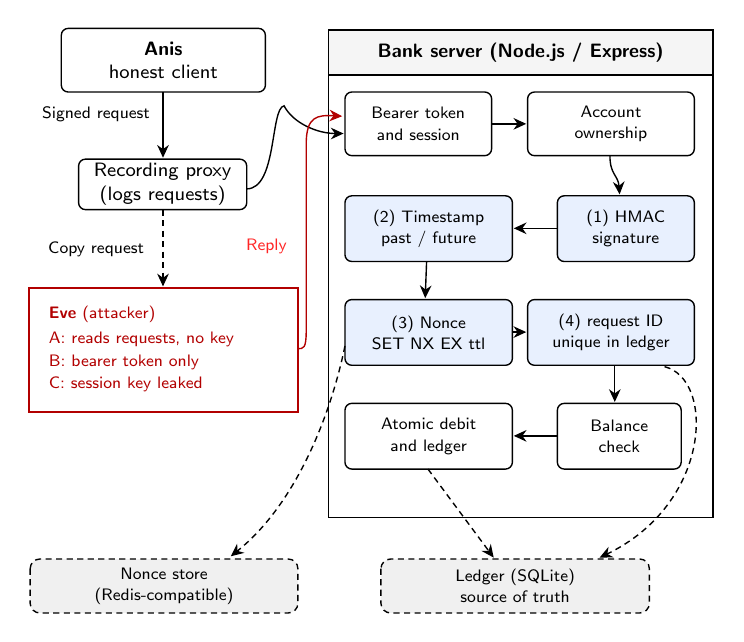
\begin{tikzpicture}[
        x=0.25pt, y=-0.25pt,
        font=\sffamily\fontsize{6.5}{7.7}\selectfont,
        box/.style={draw=black, line width=0.5pt, rounded corners=2.5pt, align=center, inner sep=0pt, fill=white},
        stage/.style={box, fill={rgb,255:red,232;green,240;blue,254}},
        store/.style={box, dashed, dash pattern=on 2.2pt off 1.6pt, rounded corners=3.5pt, fill={rgb,255:red,240;green,240;blue,240}},
        flow/.style={-{Stealth[length=4.6pt,width=4.2pt]}, line width=0.5pt},
        dflow/.style={flow, dash pattern=on 2.2pt off 1.6pt},
        rflow/.style={-{Stealth[length=4.6pt,width=4.2pt]}, line width=0.5pt, color=red!70!black}
    ]
    % ---------- left column ----------
    \draw[box] (50,3) rectangle (345,95) node[midway,font=\sffamily\fontsize{7.2}{8.6}\selectfont] {\textbf{Anis}\\honest client};
    \draw[box] (75,192) rectangle (318,265) node[midway,font=\sffamily\fontsize{7.2}{8.6}\selectfont] {Recording proxy\\(logs requests)};
    \node[anchor=west] at (8,128) {Signed request};
    \node[anchor=west] at (17,322) {Copy request};
    \node[anchor=west,text=red!85!white] at (303,318) {Reply};

    % Eve
    \draw[red!70!black, line width=0.8pt] (3,378) rectangle (392,558);
    \node[anchor=west,text=red!70!black] at (18,416) {\textbf{Eve} (attacker)};
    \node[anchor=west,text=red!70!black] at (18,453) {A: reads requests, no key};
    \node[anchor=west,text=red!70!black] at (18,486) {B: bearer token only};
    \node[anchor=west,text=red!70!black] at (18,517) {C: session key leaked};

    % ---------- bank server ----------
    \draw[line width=0.6pt, fill=white] (436,5) rectangle (992,710);
    \draw[line width=0.6pt, fill=black!4] (436,5) rectangle (992,70);
    \node[font=\sffamily\fontsize{7.4}{8.6}\selectfont\bfseries] at (714,38) {Bank server (Node.js / Express)};

    \draw[box]   (460,95)  rectangle (672,187) node[midway] (bearer) {Bearer token\\and session};
    \draw[box]   (724,95)  rectangle (965,187) node[midway] {Account\\ownership};
    \draw[stage] (460,245) rectangle (702,340) node[midway] {(2) Timestamp\\past / future};
    \draw[stage] (767,245) rectangle (965,340) node[midway] {(1) HMAC\\signature};
    \draw[stage] (460,395) rectangle (702,490) node[midway] {(3) Nonce\\SET NX EX ttl};
    \draw[stage] (724,395) rectangle (965,490) node[midway] {(4) request ID\\unique in ledger};
    \draw[box]   (460,545) rectangle (702,640) node[midway] {Atomic debit\\and ledger};
    \draw[box]   (767,545) rectangle (946,640) node[midway] {Balance\\check};

    % ---------- stores ----------
    \draw[store] (5,770)   rectangle (392,848) node[midway] {Nonce store\\(Redis-compatible)};
    \draw[store] (512,770) rectangle (900,848) node[midway] {Ledger (SQLite)\\source of truth};

    % ---------- solid flow ----------
    \draw[flow] (197,95) -- (197,190);
    \draw[flow, dash pattern=on 2.2pt off 1.6pt] (197,265) -- (197,376);
    \draw[flow] (318,235) .. controls (362,235) and (352,118) .. (372,115)
        .. controls (385,140) and (420,155) .. (458,155);
    \draw[rflow] (392,466) .. controls (400,466) and (404,466) .. (404,440)
        -- (404,170) .. controls (404,130) and (420,128) .. (456,130);
    \draw[flow] (672,141) -- (722,141);
    \draw[flow] (843,187) .. controls (843,215) and (855,215) .. (857,243);
    \draw[flow] (767,292) -- (704,292);
    \draw[flow] (578,340) -- (576,393);
    \draw[flow] (702,442) -- (722,442);
    \draw[flow] (850,490) -- (850,543);
    \draw[flow] (767,592) -- (704,592);

    % ---------- dashed (state) flow ----------
    \draw[dflow] (460,462) .. controls (440,560) and (390,690) .. (295,766);
    \draw[dflow] (922,492) .. controls (995,510) and (990,690) .. (828,768);
    \draw[dflow] (580,640) -- (675,768);
    \end{tikzpicture}
    \caption{Threat model and bank server request-validation workflow.}
    \label{fig:pipeline}
\end{figure}



\subsection{Testbed and request pipeline}
We have a small testbed with a banking API (Fig.~\ref{fig:pipeline}), which is implemented with a Node.js/Express server providing the login, withdraw, and deposit functionalities. The accounts and ledger information are stored in SQLite. The nonces are stored in Redis-compatible storage (Memurai 4.2.3, Windows).

During login (user ID + PIN), the server provides a bearer token and a secret session key $K_s$, which is not retransmitted later. All requests contain the token and: method, path, user ID, account ID, amount, currency, timestamp, nonce, request ID, and signature. Signature is calculated as HMAC-SHA256 on all other parameters using $K_s$. It is our own implementation, not RFC 9421 and DPoP, although based on these. Fields that contain ``$|$'' or control characters are rejected.

Once token ownership validation is completed, there are four additional stages of protocol flow. These stages are denoted H, T, N, and R respectively. \textbf{H} (signature) is stage during which HMAC hash is recomputed and compared. \textbf{T} (timestamp) is stage of timestamp verification; which allows maximum PAST clock time in seconds from the transaction which occurred earlier and maximum FUTURE clock time in seconds until the transaction takes place (default values are 300 sec and 5 sec respectively). \textbf{N} (nonce) is nonce verification stage; nonce is stored with TTL or time to live limit of a certain duration (default is 300 sec). Finally \textbf{R} (request ID) is ID verification which looks up the ID stored in the ledger and any duplicates are rejected. H1T0N1R0 means that only H and N are on, all other stages are off. 

\subsection{Threat model and attack scenarios}
The adversary is called Eve. The attacker A can alter any field in a request including token (from proxy logs or through intermediaries like proxies/gateways stripping out TLS the protocol for Web encryption) but does not know the session key and thus cannot generate a valid signature. Within the test-bed environment, Eve replays only those request that are recorded within the localhost proxy. The attacker B knows only bearer token while the attacker C knows both the session key as well. Out of scope for this research would be compromised clients, denial-of-service attacks, PIN guessing, and multi server architecture. A successful attack results when there is an additional SUCCESS withdrawal transaction on the ledger. Table~\ref{tab:attacks} lists the scenarios.

\begin{table}[!t]
\caption{Attack scenarios and number $n$ of trials per configuration (S10: 30 independent failed requests).}
\label{tab:attacks}
\centering
\scriptsize
\renewcommand{\arraystretch}{1.1}
\setlength{\tabcolsep}{3pt}
\begin{tabular}{@{}l p{2.3in} r@{}}
\toprule
ID & Eve's action & $n$ \\
\midrule
S1 & Resend a captured request immediately & 30 \\
S2 & Resend after 2 s (inside the window) & 30 \\
S3 & Clear the nonce store, then resend & 30 \\
S4 & Resend after 7 s (outside the 6 s window) & 30 \\
S5 & Send 50 identical copies in parallel, 30 batches & 1,500 \\
S6 & Change the amount, keep the old signature & 30 \\
S7a, S7b & Change request ID (a) or nonce (b), keep the old signature & 30 each \\
S8 & Resend after the session expired & 30 \\
S9 & Attacker C: new request signed with the leaked key & 30 \\
S10 & Keep failed (insufficient balance) requests; after a deposit, replay each once, 1 s (fast) or 9 s (late) later & 30 \\
S11 & Attacker B: token only, fresh nonce, request ID and timestamp, no signature & 100 \\
\bottomrule
\end{tabular}
\end{table}

\subsection{Experiments}
\textbf{Coverage experiment (E1).} We test each of the 16 combinations of on/off for the 4 layers in all scenarios in Table II, using different servers and databases. Since it is impractical to wait 300 seconds for each experiment, the coverage experiment and retention experiment used scaled parameters: PAST 6 seconds, FUTURE 2 seconds, nonce TTL 8 seconds, session duration 15 seconds. In other runs of the same experiment, normal parameters were employed. The result was consistent for all trials, and we report results with 95\% Wilson confidence intervals (0 out of 30 corresponds to true rate not greater than 11.4\%; 0 out of 100 means not more than 3.7\%).

\textbf{Failed request experiment (S10).} There are 30 failed attempts to withdraw 100 amount of money every time with an INSUFFICIENT\_BALANCE error. The balance at this time is 1. In the next phase, a deposit of 3001 is made to the account. Eve replays every failed request after 1 second (fast) or 9 seconds (slow) after making a deposit, according to the two policies. In \ao{} case, retries are made in two possible ways- either with same ID and new nonce or with different and new ID (Fig.~\ref{fig:s10}).

\begin{figure}[!t]
\centering
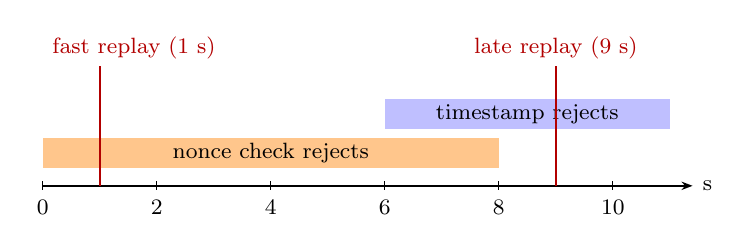
\begin{tikzpicture}[x=0.285in,y=0.75in,font=\footnotesize]
  \draw[-{Stealth[length=4pt]},thick] (0,0) -- (11.4,0) node[right,font=\footnotesize]{s};
  \foreach \x in {0,2,4,6,8,10} {\draw (\x,0.03) -- (\x,-0.03); \node[below,font=\footnotesize] at (\x,-0.03) {\x};}
  \fill[orange!45] (0,0.12) rectangle (8,0.32); \node[font=\footnotesize] at (4,0.22) {nonce check rejects};
  \fill[blue!25] (6,0.38) rectangle (11,0.58); \node[font=\footnotesize] at (8.5,0.48) {timestamp rejects};
  \draw[thick,red!70!black] (1,0) -- (1,0.8); \node[above,red!70!black,align=center,font=\footnotesize] at (1.6,0.78) {fast replay (1 s)};
  \draw[thick,red!70!black] (9,0) -- (9,0.8); \node[above,red!70!black,align=center,font=\footnotesize] at (9,0.78) {late replay (9 s)};
\end{tikzpicture}
\caption{S10 timeline (scaled settings, schematic). Eve copies a failed request, a deposit follows, then Eve replays it. Orange: the nonce is still remembered (8 s). Blue: the request is older than the 6 s past limit. A fast replay is stopped only by the nonce check, a late replay only by the timestamp check. Delays are counted from the deposit; the failed requests were sent just before it.}
\label{fig:s10}
\end{figure}

\textbf{Retention test (E4a).} With H, T and N functioning, we change the nonce TTL (4, 6, 8, 10, 12 s), the time difference of the client clock f (0, 1, 2 s) and the delay time $d$ (1, 3, 5, 6, 7, 8, 9, 10, 11 s), conducting 30 trials for each delay. After reaching the point when $d \ge \mathrm{TTL}$, the nonce no longer exists in memory. Nevertheless, until $d < \mathrm{PAST}+f$, the request still seems to be new, as the clock ahead by $f$ seconds makes the request appear new. So a replay succeeds exactly when
\begin{equation}
\mathrm{TTL} \le d < \mathrm{PAST} + f,
\label{eq:gap}
\end{equation}
When the nonce TTL is at least PAST + FUTURE, the gap in Eq.~(\ref{eq:gap}) closes. For the full-scale check, we used the default settings (TTL 300 s, PAST 300 s, FUTURE 5 s), with the client clock 4 s ahead and replay delays of 299, 301, 303, 305 and 307 s, with R on and off.

\textbf{Cost testing (E2).} in eight variations: none, with H, with H and T, with H and T and N, and so forth (in total, all possible combinations), with the total of 10 repetitions per each case (in which the time is recorded in the server).

\textbf{Test of clock-error (E3).} 
It simulates genuine requests. The time-stamped sending time (i.e., when the request message is sent) is computed by adding the offset of the client clock. The server gets the message after some delay. The stage of the request at the server is given by the following formula: $\text{delay} - \text{offset}$. The server accepts this request when $-\mathrm{FUTURE} \le \text{age} \le \mathrm{PAST}$. Types of requests with time periods of PAST $\in\{5,30,60,120,300\}$ s, and FUTURE $\in\{0,2,5,30,60\}$ s are included in combinations with three alternative profiles containing a total of 75 cells and the number of requests. The delays are log-normally distributed according to the certain profile. The offset is normal, $N(0,\sigma)$; the delay is log-normal with a median and a shape. P1: $\sigma=0.5$ s, median 0.2 s, shape 0.6. P2: 3 s, 0.5 s, 1.0. P3: 30 s, 2 s, 1.2. Each cell draws its own requests, so differences below about one percentage point are noise.

\textbf{Testing Failure (E4b, E4c).} The nonce store is disrupted through a route that tests only cases with 30 honest requests and 30 replays each. When a response goes missing from the server, the transaction will process but the client will not receive the information and abort the attempt. Each cell will consist of 200 transactions during which responses are discarded with proportions $p=0$, 0.05 and 0.2, in the order given or by the request ID provided, while the nonce is the same or different in retries. 

\textbf{Additional Tests.} We also conducted a witness group of honest requests and checked for route binding and atomic debit as well as reporting any time-based issues present in the testing phase. To this end, the testing harness contains 44 tests and a separate analysis script whereby 4,532 values were computed with no differences observed. The code and data can be found here: \href{https://github.com/shahriarshad/Replay-Attack-Simulation}{\texttt{github.com/\allowbreak shahriarshad/\allowbreak Replay-Attack-Simulation}}.

\section{Results}\label{sec:results}

\subsection{Coverage of the four layers (E1)}
\textbf{Question:} which attacks does each layer block? \textbf{Answer:} no single layer can block all attacks; however, when the four layers are used together, all attacks can be blocked except the one involving key leakage (S9)  (see Fig.~\ref{fig:heat}).H does not block replay attacks (S1 through S5 are not blocked by H alone (H1T0N0R0)), but H is effective in blocking S11. Both S6 and S7a and S7b use other identifiers, meaning that N or R can also stop them. N is effective in stopping S1, S2, and S5 and, given that TTL can go back to PAST, S4 too. S3 cannot be stopped though, and it is bypassed by the new nonce once H is turned off (S7b). T only stops S4 and the late S10. R stops S1 through S6, but S7a cannot be stopped without H, and \so{} means S10 is not stopped. H plus R stop everything except S9 and S10. S8 was 0/30 and S9 was 30/30 irrespective of the configuration. Honest control requests were accepted 30/30 in all configurations.



\begin{figure}[!t]
\centering
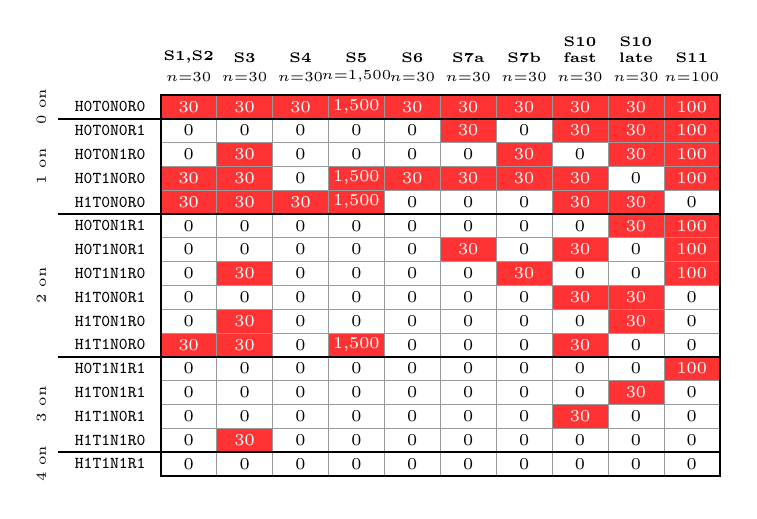
\begin{tikzpicture}[x=1pt,y=-1pt,font=\fontsize{6}{7}\selectfont]
  % geometry: grid starts at X0=40pt, cell 20.2 x 8.6 pt
  \def\cw{20.2}\def\rh{8.6}\def\xz{40}
  % column headers
  \foreach \h/\nn [count=\c] in {{S1,S2}/30, S3/30, S4/30, S5/1{,}500, S6/30, S7a/30, S7b/30, S10\\fast/30, S10\\late/30, S11/100}{
    \node[anchor=south,align=center,font=\fontsize{5.5}{6}\selectfont\bfseries] at ({\xz+(\c-0.5)*\cw},-8) {\h};
    \node[anchor=south,font=\fontsize{4.5}{5}\selectfont,text=black] at ({\xz+(\c-0.5)*\cw},-1.2) {$n$=\nn};
  }
  % rows
  \foreach \lab/\vals [count=\r] in {
    H0T0N0R0/{30,30,30,1500,30,30,30,30,30,100},
    H0T0N0R1/{0,0,0,0,0,30,0,30,30,100},
    H0T0N1R0/{0,30,0,0,0,0,30,0,30,100},
    H0T1N0R0/{30,30,0,1500,30,30,30,30,0,100},
    H1T0N0R0/{30,30,30,1500,0,0,0,30,30,0},
    H0T0N1R1/{0,0,0,0,0,0,0,0,30,100},
    H0T1N0R1/{0,0,0,0,0,30,0,30,0,100},
    H0T1N1R0/{0,30,0,0,0,0,30,0,0,100},
    H1T0N0R1/{0,0,0,0,0,0,0,30,30,0},
    H1T0N1R0/{0,30,0,0,0,0,0,0,30,0},
    H1T1N0R0/{30,30,0,1500,0,0,0,30,0,0},
    H0T1N1R1/{0,0,0,0,0,0,0,0,0,100},
    H1T0N1R1/{0,0,0,0,0,0,0,0,30,0},
    H1T1N0R1/{0,0,0,0,0,0,0,30,0,0},
    H1T1N1R0/{0,30,0,0,0,0,0,0,0,0},
    H1T1N1R1/{0,0,0,0,0,0,0,0,0,0}}{
    \node[anchor=east,text=black,font=\fontsize{5.6}{6.5}\selectfont\ttfamily] at ({\xz-2},{(\r-0.5)*\rh}) {\lab};
    \foreach \v [count=\c] in \vals {
      \ifnum\v>0 \def\fc{red!80!white}\def\tc{white}\else\def\fc{white}\def\tc{black}\fi
      \path[fill=\fc,draw=black!40,line width=0.2pt] ({\xz+(\c-1)*\cw},{(\r-1)*\rh}) rectangle ({\xz+\c*\cw},{\r*\rh});
      \node[text=\tc] at ({\xz+(\c-0.5)*\cw},{(\r-0.5)*\rh}) {\ifnum\v=1500 1{,}500\else\v\fi};
    }
  }
  % group separators and outer frame
  \foreach \r in {1,5,11,15}{\draw[line width=0.7pt] ({\xz-37},{\r*\rh}) -- ({\xz+10*\cw},{\r*\rh});}
  \draw[line width=0.7pt] (\xz,0) rectangle ({\xz+10*\cw},{16*\rh});
  % group labels
  \node[anchor=south,font=\fontsize{5}{6}\selectfont,text=black,rotate=90] at (2,{0.5*\rh}) {0 on};
  \node[anchor=south,font=\fontsize{5}{6}\selectfont,text=black,rotate=90] at (2,{3*\rh}) {1 on};
  \node[anchor=south,font=\fontsize{5}{6}\selectfont,text=black,rotate=90] at (2,{8*\rh}) {2 on};
  \node[anchor=south,font=\fontsize{5}{6}\selectfont,text=black,rotate=90] at (2,{13*\rh}) {3 on};
  \node[anchor=south,font=\fontsize{5}{6}\selectfont,text=black,rotate=90] at (2,{15.5*\rh}) {4 on};
\end{tikzpicture}
\caption{Coverage matrix (E1): successful attacks out of $n$ trials for all 16 configurations (H = HMAC, T = timestamp, N = nonce, R = request ID; 1 = on). Red means at least one attack succeeded; the number is the count. Scaled profile (PAST 6 s, FUTURE 2 s, nonce TTL 8 s), policy \so{}. S8 (0/30) and S9 (30/30) are identical in all rows and omitted.}
\label{fig:heat}
\end{figure}

\subsection{The failed-request replay and idempotency policy (S10)}
\textbf{Question:} The question is whether the failed-request policy determines if a replay is valid after the account has been credited. \textbf{Answer:} The answer is in(Table~\ref{tab:s10}). \so{} provides no protection against S10: with N and T disabled, all 30 failed requests were executed after the deposit, irrespective of how fast or slow these requests were (Wilson interval [0.886, 1.000]). N alone is effective against fast replays (the nonce has expired), T alone against slow ones, while both N and T together are effective against either type. Under \ao{}, the protection of R is absolute (0/30). We also ran S10 for all 16 layer configurations under both policies; under \ao{}, every configuration with R on blocked both fast and late replays (0/30).

\begin{table}[!t]
\caption{S10: executed replays of 30 failed requests by policy and layers (top; H and R any), and retries with a new nonce after the deposit, accepted of 30 (bottom).}
\label{tab:s10}
\centering
\footnotesize
\setlength{\tabcolsep}{4pt}
\begin{tabular}{@{}llcc@{}}
\toprule
Policy & Layers on & Fast & Late \\
\midrule
\so & N, T off & 30/30 & 30/30 \\
\so & T only & 30/30 & 0/30 \\
\so & N only & 0/30 & 30/30 \\
\so & N and T & 0/30 & 0/30 \\
\ao & R on & 0/30 & 0/30 \\
\midrule
 & & Same ID & New ID \\
\midrule
\so & & 30/30 & 30/30 \\
\ao & & 0/30 & 30/30 \\
\bottomrule
\end{tabular}
\end{table}

\subsection{Nonce retention and timestamp window (E4a)}
\textbf{Question:} What is the required retention time of a nonce? 
\textbf{Answer:} The value for nonce retention must be at a minimum of PAST + FUTURE. All 30, 60, 90 successful replays out of 270 were recorded in case the R is off at TTL 4 s (f = 0, 1, 2 s) while all 0, 30, 60 successful replays were recorded at TTL 6 s and 0 for TTL 8, 10 and 12 s. Meanwhile, with R on, all replays were recorded as 0. Rule~(\ref{eq:gap}) fulfilled the requirement of 135 on 135 cases. Also, in the full run with R off (Fig.~\ref{fig:gap}(b)), the successful runs of 299 s were stopped because of N, 301 s and 303 s were successful (30/30), while 305 s and 307s were stopped by T. With R being activated, all five delays resulted in a 0/30 (ALREADY\_PROCESSED at 301 seconds and 303 seconds). The default TTL (at 300 seconds) corresponds to PAST and misses PAST+FUTURE by 5 seconds and the server displays a startup warning. With all four layers turned on at default parameters, replays at the 60-second mark (S2) and the 301-second mark (S4) recorded a 0/30 status.

\begin{figure}[!t]
\centering
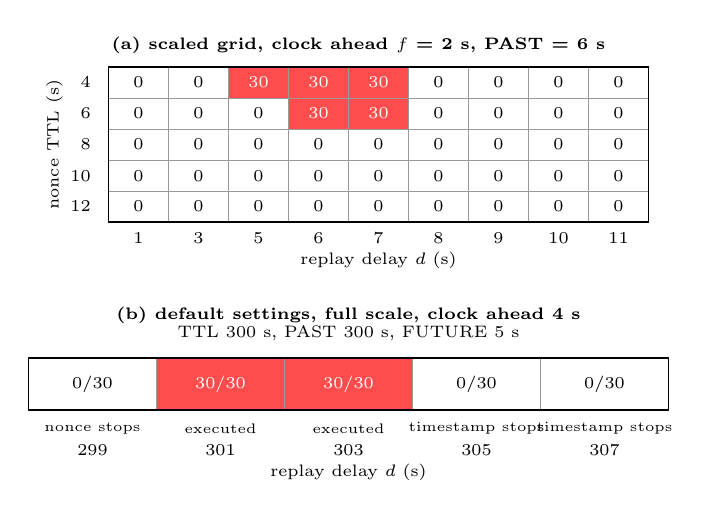
\begin{tikzpicture}[x=1in,y=1in,font=\fontsize{6}{7}\selectfont]
\node[anchor=east] at (0.480,1.998) {4};
\path[fill=white,draw=black!40,line width=0.2pt] (0.520,1.920) rectangle (0.820,2.075);
\node[text=black] at (0.670,1.998) {0};
\path[fill=white,draw=black!40,line width=0.2pt] (0.820,1.920) rectangle (1.120,2.075);
\node[text=black] at (0.970,1.998) {0};
\path[fill=red!70!white,draw=black!40,line width=0.2pt] (1.120,1.920) rectangle (1.420,2.075);
\node[text=white] at (1.270,1.998) {30};
\path[fill=red!70!white,draw=black!40,line width=0.2pt] (1.420,1.920) rectangle (1.720,2.075);
\node[text=white] at (1.570,1.998) {30};
\path[fill=red!70!white,draw=black!40,line width=0.2pt] (1.720,1.920) rectangle (2.020,2.075);
\node[text=white] at (1.870,1.998) {30};
\path[fill=white,draw=black!40,line width=0.2pt] (2.020,1.920) rectangle (2.320,2.075);
\node[text=black] at (2.170,1.998) {0};
\path[fill=white,draw=black!40,line width=0.2pt] (2.320,1.920) rectangle (2.620,2.075);
\node[text=black] at (2.470,1.998) {0};
\path[fill=white,draw=black!40,line width=0.2pt] (2.620,1.920) rectangle (2.920,2.075);
\node[text=black] at (2.770,1.998) {0};
\path[fill=white,draw=black!40,line width=0.2pt] (2.920,1.920) rectangle (3.220,2.075);
\node[text=black] at (3.070,1.998) {0};
\node[anchor=east] at (0.480,1.843) {6};
\path[fill=white,draw=black!40,line width=0.2pt] (0.520,1.765) rectangle (0.820,1.920);
\node[text=black] at (0.670,1.843) {0};
\path[fill=white,draw=black!40,line width=0.2pt] (0.820,1.765) rectangle (1.120,1.920);
\node[text=black] at (0.970,1.843) {0};
\path[fill=white,draw=black!40,line width=0.2pt] (1.120,1.765) rectangle (1.420,1.920);
\node[text=black] at (1.270,1.843) {0};
\path[fill=red!70!white,draw=black!40,line width=0.2pt] (1.420,1.765) rectangle (1.720,1.920);
\node[text=white] at (1.570,1.843) {30};
\path[fill=red!70!white,draw=black!40,line width=0.2pt] (1.720,1.765) rectangle (2.020,1.920);
\node[text=white] at (1.870,1.843) {30};
\path[fill=white,draw=black!40,line width=0.2pt] (2.020,1.765) rectangle (2.320,1.920);
\node[text=black] at (2.170,1.843) {0};
\path[fill=white,draw=black!40,line width=0.2pt] (2.320,1.765) rectangle (2.620,1.920);
\node[text=black] at (2.470,1.843) {0};
\path[fill=white,draw=black!40,line width=0.2pt] (2.620,1.765) rectangle (2.920,1.920);
\node[text=black] at (2.770,1.843) {0};
\path[fill=white,draw=black!40,line width=0.2pt] (2.920,1.765) rectangle (3.220,1.920);
\node[text=black] at (3.070,1.843) {0};
\node[anchor=east] at (0.480,1.688) {8};
\path[fill=white,draw=black!40,line width=0.2pt] (0.520,1.610) rectangle (0.820,1.765);
\node[text=black] at (0.670,1.688) {0};
\path[fill=white,draw=black!40,line width=0.2pt] (0.820,1.610) rectangle (1.120,1.765);
\node[text=black] at (0.970,1.688) {0};
\path[fill=white,draw=black!40,line width=0.2pt] (1.120,1.610) rectangle (1.420,1.765);
\node[text=black] at (1.270,1.688) {0};
\path[fill=white,draw=black!40,line width=0.2pt] (1.420,1.610) rectangle (1.720,1.765);
\node[text=black] at (1.570,1.688) {0};
\path[fill=white,draw=black!40,line width=0.2pt] (1.720,1.610) rectangle (2.020,1.765);
\node[text=black] at (1.870,1.688) {0};
\path[fill=white,draw=black!40,line width=0.2pt] (2.020,1.610) rectangle (2.320,1.765);
\node[text=black] at (2.170,1.688) {0};
\path[fill=white,draw=black!40,line width=0.2pt] (2.320,1.610) rectangle (2.620,1.765);
\node[text=black] at (2.470,1.688) {0};
\path[fill=white,draw=black!40,line width=0.2pt] (2.620,1.610) rectangle (2.920,1.765);
\node[text=black] at (2.770,1.688) {0};
\path[fill=white,draw=black!40,line width=0.2pt] (2.920,1.610) rectangle (3.220,1.765);
\node[text=black] at (3.070,1.688) {0};
\node[anchor=east] at (0.480,1.532) {10};
\path[fill=white,draw=black!40,line width=0.2pt] (0.520,1.455) rectangle (0.820,1.610);
\node[text=black] at (0.670,1.532) {0};
\path[fill=white,draw=black!40,line width=0.2pt] (0.820,1.455) rectangle (1.120,1.610);
\node[text=black] at (0.970,1.532) {0};
\path[fill=white,draw=black!40,line width=0.2pt] (1.120,1.455) rectangle (1.420,1.610);
\node[text=black] at (1.270,1.532) {0};
\path[fill=white,draw=black!40,line width=0.2pt] (1.420,1.455) rectangle (1.720,1.610);
\node[text=black] at (1.570,1.532) {0};
\path[fill=white,draw=black!40,line width=0.2pt] (1.720,1.455) rectangle (2.020,1.610);
\node[text=black] at (1.870,1.532) {0};
\path[fill=white,draw=black!40,line width=0.2pt] (2.020,1.455) rectangle (2.320,1.610);
\node[text=black] at (2.170,1.532) {0};
\path[fill=white,draw=black!40,line width=0.2pt] (2.320,1.455) rectangle (2.620,1.610);
\node[text=black] at (2.470,1.532) {0};
\path[fill=white,draw=black!40,line width=0.2pt] (2.620,1.455) rectangle (2.920,1.610);
\node[text=black] at (2.770,1.532) {0};
\path[fill=white,draw=black!40,line width=0.2pt] (2.920,1.455) rectangle (3.220,1.610);
\node[text=black] at (3.070,1.532) {0};
\node[anchor=east] at (0.480,1.378) {12};
\path[fill=white,draw=black!40,line width=0.2pt] (0.520,1.300) rectangle (0.820,1.455);
\node[text=black] at (0.670,1.378) {0};
\path[fill=white,draw=black!40,line width=0.2pt] (0.820,1.300) rectangle (1.120,1.455);
\node[text=black] at (0.970,1.378) {0};
\path[fill=white,draw=black!40,line width=0.2pt] (1.120,1.300) rectangle (1.420,1.455);
\node[text=black] at (1.270,1.378) {0};
\path[fill=white,draw=black!40,line width=0.2pt] (1.420,1.300) rectangle (1.720,1.455);
\node[text=black] at (1.570,1.378) {0};
\path[fill=white,draw=black!40,line width=0.2pt] (1.720,1.300) rectangle (2.020,1.455);
\node[text=black] at (1.870,1.378) {0};
\path[fill=white,draw=black!40,line width=0.2pt] (2.020,1.300) rectangle (2.320,1.455);
\node[text=black] at (2.170,1.378) {0};
\path[fill=white,draw=black!40,line width=0.2pt] (2.320,1.300) rectangle (2.620,1.455);
\node[text=black] at (2.470,1.378) {0};
\path[fill=white,draw=black!40,line width=0.2pt] (2.620,1.300) rectangle (2.920,1.455);
\node[text=black] at (2.770,1.378) {0};
\path[fill=white,draw=black!40,line width=0.2pt] (2.920,1.300) rectangle (3.220,1.455);
\node[text=black] at (3.070,1.378) {0};
\node at (0.670,1.220) {1};
\node at (0.970,1.220) {3};
\node at (1.270,1.220) {5};
\node at (1.570,1.220) {6};
\node at (1.870,1.220) {7};
\node at (2.170,1.220) {8};
\node at (2.470,1.220) {9};
\node at (2.770,1.220) {10};
\node at (3.070,1.220) {11};
\node at (1.870,1.110) {replay delay $d$ (s)};
\node[rotate=90] at (0.250,1.688) {nonce TTL (s)};
\draw[line width=0.6pt] (0.520,1.300) rectangle (3.220,2.075);
\node[font=\fontsize{6.5}{7.5}\selectfont\bfseries] at (1.770,2.185) {(a) scaled grid, clock ahead $f$ = 2 s, PAST = 6 s};
\path[fill=white,draw=black!40,line width=0.2pt] (0.120,0.360) rectangle (0.760,0.620);
\node[text=black] at (0.440,0.490) {0/30};
\node[font=\fontsize{5}{6}\selectfont] at (0.440,0.270) {nonce stops};
\node at (0.440,0.160) {299};
\path[fill=red!70!white,draw=black!40,line width=0.2pt] (0.760,0.360) rectangle (1.400,0.620);
\node[text=white] at (1.080,0.490) {30/30};
\node[font=\fontsize{5}{6}\selectfont] at (1.080,0.270) {executed};
\node at (1.080,0.160) {301};
\path[fill=red!70!white,draw=black!40,line width=0.2pt] (1.400,0.360) rectangle (2.040,0.620);
\node[text=white] at (1.720,0.490) {30/30};
\node[font=\fontsize{5}{6}\selectfont] at (1.720,0.270) {executed};
\node at (1.720,0.160) {303};
\path[fill=white,draw=black!40,line width=0.2pt] (2.040,0.360) rectangle (2.680,0.620);
\node[text=black] at (2.360,0.490) {0/30};
\node[font=\fontsize{5}{6}\selectfont] at (2.360,0.270) {timestamp stops};
\node at (2.360,0.160) {305};
\path[fill=white,draw=black!40,line width=0.2pt] (2.680,0.360) rectangle (3.320,0.620);
\node[text=black] at (3.000,0.490) {0/30};
\node[font=\fontsize{5}{6}\selectfont] at (3.000,0.270) {timestamp stops};
\node at (3.000,0.160) {307};
\node at (1.720,0.050) {replay delay $d$ (s)};
\draw[line width=0.6pt] (0.120,0.360) rectangle (3.320,0.620);
\node[font=\fontsize{6.5}{7.5}\selectfont\bfseries,align=center] at (1.720,0.790) {(b) default settings, full scale, clock ahead 4 s\\[-1pt]\fontsize{6}{7}\selectfont\mdseries TTL 300 s, PAST 300 s, FUTURE 5 s};
\end{tikzpicture}
\caption{Nonce retention gap (E4a): replays executed out of 30 per cell (red), R off. (a) Scaled grid, client clock 2 s ahead: replays succeed for TTL $\le d <$ PAST $+ f$. (b) Default settings at full scale, clock 4 s ahead: replays succeed between 300 s and 304 s.}
\label{fig:gap}
\end{figure}

\subsection{Layers Cost (E2)}
\textbf{Question:} what are the costs of the layers? \textbf{Answer:} In essence, the cost of the layers is around 0.5 ms per request, split mainly between the request-ID lookup (240 $\mu$s) and the nonce store (190 $\mu$s) (Table~\ref{tab:cost}).The four layers' own time sums to 0.48 ms and the end-to-end handler time rises by 0.62 ms (6.07 to 6.69 ms, around 10\%; a repeat run gave 6.67 ms), because the second request-ID check is not included in the per-layer sum. Rejected requests are much cheaper than accepted ones: wrong signature 0.73 ms, stale timestamp 0.72 to 0.78 ms, duplicate nonce 0.94 to 1.27 ms, duplicate request ID 1.06 to 1.28 ms, versus 6 to 7 ms for an accepted request.The numbers presented are for comparative purposes only.



\begin{table}[!t]
\caption{Cost (E2): server handler time (ms, median of repeat medians) and per-layer time ($\mu$s, all four layers on).}
\label{tab:cost}
\centering
\footnotesize
\setlength{\tabcolsep}{4pt}
\begin{tabular}{@{}lrlr@{}}
\toprule
Configuration & ms & Layer (own time) & $\mu$s \\
\midrule
None & 6.07 & HMAC & 37 \\
H & 6.13 & Timestamp & 10 \\
H+T & 6.13 & Nonce (Redis-compat.) & 190 \\
H+T+N & 6.32 & request ID & 240 \\
All four & 6.69 & Sum & 477 \\
All four, memory nonce & 6.45 & Nonce, memory & 16 \\
All four, SQLite nonce & 11.22 & Nonce, SQLite & 4,517 \\
\bottomrule
\end{tabular}
\end{table}

\subsection{False rejection of honest customers (E3)}
\textbf{Question:} what is the number of honest clients that are wrongly rejected? \textbf{Answer:} around one third at FUTURE = 0; small FUTURE corrects it, but small PAST rejects clients due to their slow clocks. At FUTURE = 0 the rejection rate varied between 31\% - 33\%, although the clients were well synchronized using profile P1 since being a little too fast is interpreted as future; however, by setting FUTURE to 2 seconds or longer this particular issue was resolved. In the case of severe profile P3, with PAST = 300 s and FUTURE = 5 s, the rejection was 38.9\%, while with FUTURE set to 60 s the rejection dropped to 0.95\% (19 of 2,000 requests, P3, PAST = 300 s).

\subsection{Malfunction behavior (E4b, E4c) }
\textbf{Question:} what do we do when the nonce store fails or the response is lost? \textbf{Answer:} the fail-open mode lets service continue to operate but lets replays through unless R is turned on. When responses are lost nothing is charged twice but the error may not be obvious (as can be seen from (Table~\ref{tab:fail})). If the store fails while R is off, the fail-open mode lets all 30 requests go through successfully while fail-closed rejects all legitimate requests and all replays. When responses are lost, each request ID is charged only once (200 requests from 200) for 0, 10 and 40 lost responses.With the default ordering and a perfect retry the error message was NONCE FAIL so the client could not tell that the prior request had succeeded (0 of 10, 0 of 40). With R first or a new-nonce retry the error message was ALREADY\_PROCESSED allowing the client to know that the earlier request had been successful (success inferable in 10 of 10 and 40 of 40 retries).



\begin{table}[!t]
\caption{Failure behaviour: nonce-store failure (E4b, 30 legitimate requests and 30 replays) and lost responses (E4c, 10 and 40 lost).}
\label{tab:fail}
\centering
\footnotesize
\setlength{\tabcolsep}{3pt}
\begin{tabular}{@{}llcc@{}}
\toprule
Mode & R & Legit. accepted & Replay succeeded \\
\midrule
Fail-open & off & 30/30 & 30/30 \\
Fail-open & on & 30/30 & 0/30 \\
Fail-closed & off or on & 0/30 & 0/30 \\
\midrule
\multicolumn{2}{l}{Lost response, retry} & Error & Success inferable \\
\midrule
\multicolumn{2}{l}{Default order, identical} & NONCE\_FAIL & 0 of 10 / 0 of 40 \\
\multicolumn{2}{l}{R first, or new nonce} & ALREADY\_PROC. & 10 of 10 / 40 of 40 \\
\bottomrule
\end{tabular}
\end{table}

\subsection{Correctness and resource checks}
In the correctness and resource validation tests, a signed deposit sent to the withdrawal endpoint, and vice versa, was denied with HTTP status 400, rendering no ledger rows (in all 4 test cases, whether Testing was ON or OFF). With a balance of 100, 100 parallel withdrawals of 1 each were repeated 30 times without the balance going negative. There were a total of 1,000 iterations of 50 identical requests, where only one request was accepted from each batch. A request with age 299 s was accepted while a request of age 301 s was refused. A request with a timestamp of 5 s ahead was accepted whereas the request with age of 6 s ahead was rejected.

\section{Discussion and Limitations}\label{sec:disc}

\textbf{Lessons.} (i) Preserve nonce retention = PAST + FUTURE. PAST alone isn’t enough with a future tolerance. (ii) Maintain a small but non zero FUTURE tolerance, because FUTURE = 0 fails ~1/3 of honest clients with P1. (iii) Intentionally decide on an idempotency policy and also record failures (returning the same result would feel natural but has never been tested), or preserve checks both on nonce and time. (iv) Never use nonce without a signature (S7b). (v) Pick fail-open or fail-closed nonce storage and use a durable request ID layer with fail-open. (vi) Early check the request ID for unambiguous errors in case of response loss. Make sessions short-lived and keep keys secret. S9 proves that none of the layers is useful when the key leaks. The assertion of necessity of all four layers applies only to \so{}. By combining E1 (works with \so{}) and S10, our results suggest that \ao{} with HMAC and request ID defeats all attacks except S9.

\textbf{Limitations.} This is a local Windows laptop emulation using Memurai (instead of Redis) for comparison. Samples are small (0/30 $\leq 11.4\%$, 0/100 $\leq 3.7\%$), although results were identical among all the experiments. E1 (S1-S9, S11) was run under \so{}; S10 was run for all 16 configurations under both policies. E1 and grid experiments use scaled time. Default-window experiments involve S2, S4, and retention window but not S10 late. Distribution of E3 is assumed. One process with transaction lock provides race results. Multi-process and distributed setups are not included. The E4b table uses 30 replays per cell. Earlier runs with one replay per cell were superseded. Tests were done using HTTP with one user, light load, no mixed traffic, and faults injected within the process.

\section{Conclusion}\label{sec:concl}
Every replay defense layer covers up a different gap, and leftover gaps are due to configuration decisions. In our setup, an idempotency layer that disregards failed requests created replayable failures unless both nonce and timestamp tests were enabled. Equal nonce lifetime to past window resulted in a replay gap of the size of the future window tolerance, at default settings. The timers of all four layers together amount to about 0.5 ms per request. The results were obtained using simulation on one machine; distributed experiments are future work.



\begin{thebibliography}{00}

\bibitem{gong92}
L.~Gong, ``A security risk of depending on synchronized clocks,'' \emph{ACM SIGOPS Oper. Syst. Rev.}, vol.~26, no.~1, 1992, doi: \href{https://doi.org/10.1145/130704.130709}{10.1145/130704.130709}.

\bibitem{rfc4120}
C.~Neuman, T.~Yu, S.~Hartman, and K.~Raeburn, ``The Kerberos network authentication service (V5),'' IETF, RFC 4120, 2005, doi: \href{https://doi.org/10.17487/RFC4120}{10.17487/RFC4120}. % TODO: read replay-cache and clock-skew sections

\bibitem{almehrej}
A.~Almehrej, L.~Freitas, and P.~Modesti, ``Account and transaction protocol of the Open Banking standard,'' in \emph{Rigorous State-Based Methods (ABZ 2020)}, Lecture Notes in Computer Science, vol.~12071. Springer, 2020, pp. 230--236, doi: \href{https://doi.org/10.1007/978-3-030-48077-6_16}{10.1007/978-3-030-48077-6\_16}. % TODO: the extracted copy did not show venue/year; confirm

\bibitem{hosseyni24}
P.~Hosseyni, R.~K\"usters, and T.~W\"urtele, ``Formal security analysis of the OpenID FAPI 2.0 family of protocols: Accompanying a standardization process,'' \emph{ACM Trans. Priv. Secur.}, vol.~28, no.~1, art.~4, 2024, doi: \href{https://doi.org/10.1145/3699716}{10.1145/3699716}. % TODO: vol. 28 may be 2025; check year

\bibitem{rfc9421}
A.~Backman, J.~Richer, and M.~Sporny, ``HTTP message signatures,'' IETF, RFC 9421, Feb. 2024, doi: \href{https://doi.org/10.17487/RFC9421}{10.17487/RFC9421}.

\bibitem{rfc9449}
D.~Fett, B.~Campbell, J.~Bradley, T.~Lodderstedt, M.~Jones, and D.~Waite, ``OAuth 2.0 demonstrating proof of possession (DPoP),'' IETF, RFC 9449, Sep. 2023, doi: \href{https://doi.org/10.17487/RFC9449}{10.17487/RFC9449}.

\bibitem{fett19}
D.~Fett, P.~Hosseyni, and R.~K\"usters, ``An extensive formal security analysis of the OpenID financial-grade API,'' in \emph{Proc. IEEE Symp. Security and Privacy}, 2019, doi: \href{https://doi.org/10.1109/SP.2019.00067}{10.1109/SP.2019.00067}.

\bibitem{lee15}
C.~Lee, S.~J. Park, A.~Kejriwal, S.~Matsushita, and J.~Ousterhout, ``Implementing linearizability at large scale and low latency,'' in \emph{Proc. 25th ACM Symp. Operating Systems Principles (SOSP)}, 2015, doi: \href{https://doi.org/10.1145/2815400.2815416}{10.1145/2815400.2815416}.

\bibitem{whitaker25}
M.~Whitaker, B.~Volckaert, and M.~Al-Naday, ``Idempotency in service mesh: For resiliency of fog-native applications in multi-domain edge-to-cloud ecosystems,'' in \emph{Proc. 15th Int. Conf. Cloud Computing and Services Science (CLOSER)}, SCITEPRESS, 2025, pp. 182--189, doi: \href{https://doi.org/10.5220/0013293900003950}{10.5220/0013293900003950}.

\bibitem{stripe}
Stripe, Inc., ``Idempotent requests,'' Stripe API Reference. [Online]. Available: \href{https://docs.stripe.com/api/idempotent\_requests}{https://docs.stripe.com/api/idempotent\_requests} (accessed Oct. 2026).

\bibitem{arta}
M.~D. Arta, ``Implementasi mekanisme autentikasi API berbasis HMAC-SHA256 dengan skema nonce dan timestamp untuk mencegah replay attack,'' Institut Teknologi Bandung, 2025, \href{https://informatika.stei.itb.ac.id/~rinaldi.munir/Kriptografi/2025-2026/Makalah2025/Makalah-IF4020-Kriptografi-2025%20(37).pdf}{Institut Teknologi Bandung}.

\bibitem{ibrahim}
N.~Ibrahim and A.~Alrajh, ``A multi-layered security framework for protecting authentication link generation APIs through integrated defence in depth mechanisms,'' \emph{Int. J. Intell. Eng. Syst.}, vol.~19, no.~5, pp. 985--1004, 2026, doi: \href{https://doi.org/10.22266/ijies2026.0531.56}{10.22266/ijies2026.0531.56}.

\bibitem{krentz24}
K.-F. Krentz and T.~Voigt, ``More lightweight, yet stronger: Revisiting OSCORE's replay protection,'' in \emph{Proc. Workshop on Security and Privacy in Standardized IoT (SDIoTSec)}, NDSS Symposium, 2024, doi: \href{https://doi.org/10.14722/sdiotsec.2024.23003}{10.14722/sdiotsec.2024.23003}.

\bibitem{li18}
L.~Li, J.~Sun, Y.~Liu, M.~Sun, and J.~S. Dong, ``A formal specification and verification framework for timed security protocols,'' \emph{IEEE Trans. Softw. Eng.}, vol.~44, no.~8, pp. 725--746, 2018, doi: \href{https://doi.org/10.1109/TSE.2017.2712621}{10.1109/TSE.2017.2712621}.

\bibitem{julaihi26}
A.~A. Julaihi \emph{et al.}, ``SELAM: Selective ECC-based lightweight authentication for the internet of medical things,'' \emph{Sci. Rep.}, vol.~16, art.~20531, 2026, doi: \href{https://doi.org/10.1038/s41598-026-53641-x}{10.1038/s41598-026-53641-x}.

\bibitem{nasiri26}
M.~A. Nasiri, E.~Chatzoglou, and G.~Kambourakis, ``QUIC-er races: HTTP/3 won't save you from TOCTOU vulnerabilities,'' \emph{Int. J. Inf. Secur.}, vol.~25, art.~83, 2026, doi: \href{https://doi.org/10.1007/s10207-026-01258-6}{10.1007/s10207-026-01258-6}.

\bibitem{tlsguard}
M.~E. Abdelhafez, S.~Ramadass, and M.~Abdelwahab, ``TLS Guard for TLS 1.3 zero round-trip time (0-RTT) in a distributed environment,'' \emph{J. King Saud Univ. Comput. Inf. Sci.}, vol.~35, art.~101797, 2023, doi: \href{https://doi.org/10.1016/j.jksuci.2023.101797}{10.1016/j.jksuci.2023.101797}.

\bibitem{jing}
C.~Jing, C.~Wang, and C.~Yan, ``Replay attack: A prevalent pattern of fraudulent online transactions,'' in \emph{Proc. 5th IEEE Int. Conf. Cyber Security and Cloud Computing}, 2018, pp. 75--82, doi: \href{https://doi.org/10.1109/CSCloud/EdgeCom.2018.00022}{10.1109/CSCloud/EdgeCom.2018.00022}. % TODO: verify 18 million transactions and recall 0.72-0.93

\end{thebibliography}


\end{document}